A monophase, steady and fully developed flow of a 
Newtonian and incompressible fluid between parallel horizontal 
plates, where the lower plate moves with \textit{$U_{bottom}$} 
velocity and the upper plate moves with \textit{$ U_{top}$}, 
is known as \textit{Couette flow}. The \ref{couette}
 presents schematically this flow and the profile of the expected velocity field.

\begin{figure}[H]
\begin{center}
\begin{tikzpicture}[scale=1.2]
 \draw [pattern=north east lines] (0,0) -- (0,-0.1) -- (5,-0.1) -- (5,0) -- cycle;
 \draw [pattern=north east lines] (0,1) -- (0,1.1) -- (5,1.1) -- (5,1) -- cycle;

 \draw [->,thick] (5.1,1)--(6,1) node[above] {$U_{top}$};
 \draw [->,thick] (-0.1,0)--(-1,0) node[below] {$U_{bottom}$};
 
 \draw [->,thick] (-4,-0.1)--(-4,1.5) node[left] {$y$};
 \draw [->,thick] (-4.1,0)--(-2.5,0) node[below] {$x$};
 
 \draw [dotted] (2.5,0.0) to (2.5,1.0);
 \draw  (1.5,0.0) to (3.5,1.0);
 
 \draw [->,thick] (2.5,0.0) to (1.5,0.0);
 \draw [->,thick] (2.5,0.15) to (1.8,0.15);
 \draw [->,thick] (2.5,0.35) to (2.2,0.35);

 \draw [->,thick] (2.5,1) to (3.5,1);
 \draw [->,thick] (2.5,0.85) to (3.2,0.85);
 \draw [->,thick] (2.5,0.65) to (2.8,0.65);
\end{tikzpicture}
\end{center}
\caption{Couette Flow}
\label{couette}
\end{figure}


\noindent
The velocity profile equation is shown below:

\begin{equation}
 u = \big[ U_{top} - U_{bottom} \big] \frac{y}{L} + U_{bottom}
\end{equation}

\medskip
\noindent
where $U_{top}$ is the top plate velocity and its value is
$U_{top} = 1$, 
$U_{bottom}$ is the bottom plate velocity and its value is
$U_{bottom} = -1$, 
$L$ is non-dimensional length
beteween the plates and its value is $L = 1$
and $y$ is the vertical coordinates and it varies beteween 
$y = \big[ 0,1 \big]$.
The domaian was discretizes using a linear triangula mesh with 
3835 nodes and 7299 elements. 

\bigskip
The \ref{velocidade couette} shows the unsteady velocity profile
when $Re=100$, in addition to the comparison between 
the numerical solution and the analytical solution 
in the steady state of the proposed problem. 
It is possible to observe that the numerical solution 
converges to the analytical solution when the flow becomes steady.

\begin{figure}[H]
     \centering
     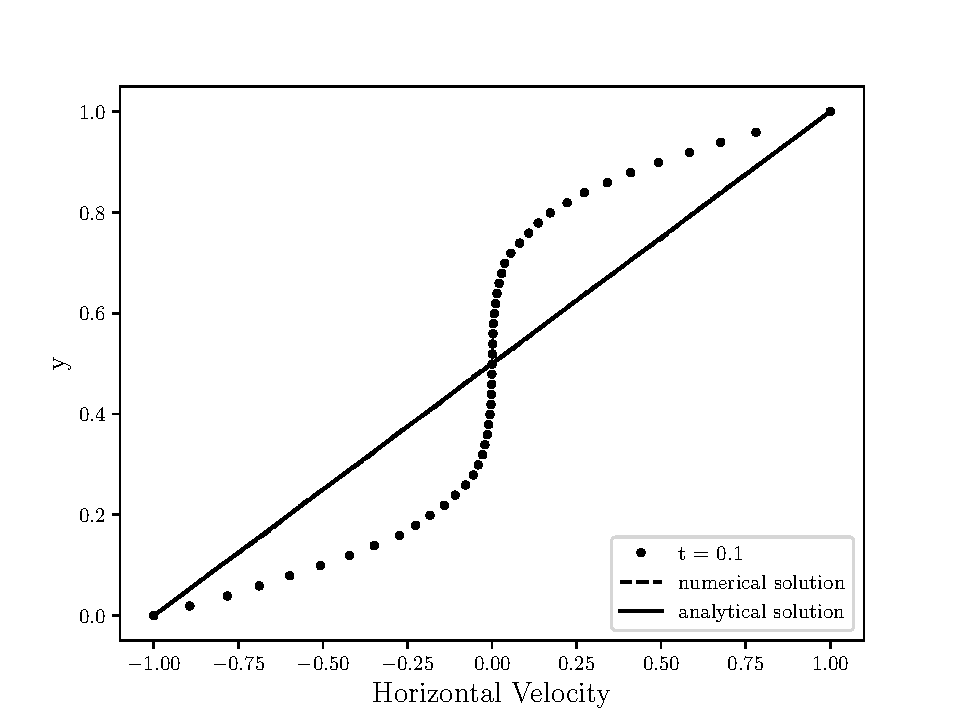
\includegraphics[scale=1]{./02_chaps/cap_validation/figure/couette_velocity.pdf}\\
     \medskip
     \caption{Unsteady velocity profile when $Re=100$ and
     the comparison beteween the numerical and analytical solution 
     for Couette flow.}
     \label{velocidade couette}
\end{figure}

\newpage
